\item[\textbf{4.}] \textbf{[20 min/20 puntos]} \textcolor{dkgreen}{Una propiedad de corrección se define como \textbf{componible} (o modular) si la validez del sistema global está garantizada siempre que cada uno de sus objetos componentes sea correcto de manera independiente. En computación concurrente, esta característica es vital para el diseño de sistemas modulares: nos permite diseñar y verificar objetos (como una Pila $A$ y una Pila $B$) por separado, con la certeza de que, al integrarlos en un mismo programa, el sistema resultante preservará dicha propiedad.}
\par
\textcolor{dkgreen}{A diferencia de otras condiciones de corrección, la \textit{linealizabilidad} es una propiedad componible. Considera, por ejemplo una ejecución $H$ cuyas proyecciones individuales son linealizables:}
\begin{itemize}
    \item \textcolor{blue}{ $H|A = push(x) \rightarrow pop():x$ }
    \item \textcolor{blue}{ $H|B = push(y) \rightarrow pop():y$ }
\end{itemize}
\textcolor{dkgreen}{Debido a que la linealizabilidad es modular, la historia global $H$ es linealizable si existe una historia secuencial legal S que respete el orden de tiempo real de todas las operaciones. En este caso, la historia $S$ resultante es:}
\begin{equation*}
    \textcolor{blue}{ S=A.push(x) < B.push(y)<B.pop():y<A.pop():x }
\end{equation*}
\begin{figure}[H]
    \centering
    \vspace{-10pt}
    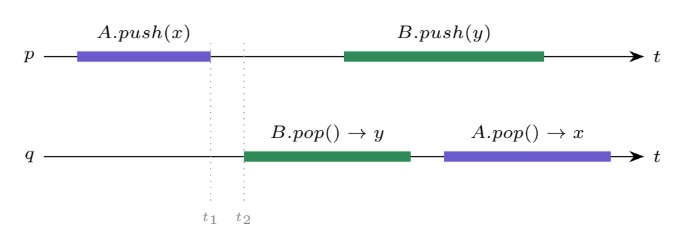
\includegraphics[width=0.8\textwidth]{Imagenes/image-2.png}
    \vspace{-10pt}
\end{figure}
\textcolor{dkgreen}{Considera dos pilas $A$ y $B$. Analiza la siguiente historia $H$:}
\begin{figure}[H]
    \centering
    \vspace{-10pt}
    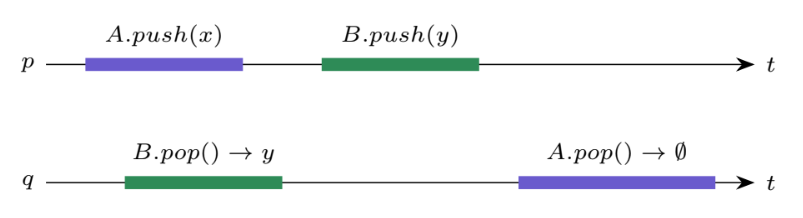
\includegraphics[width=0.8\textwidth]{Imagenes/image-3.png}
    \vspace{-10pt}
\end{figure}
\begin{enumerate}
    \item \textcolor{dkgreen}{¿Es $H|A$ secuencialmente consistente? (Pista: Busca un orden global).}
\end{enumerate}
Para la subhistoria $H|A$, solo consideramos la proyección sobre la pila $A$, es decir, la operación $A.push(x)$ del hilo $p$, y la operación $A.pop()\rightarrow\emptyset$ del hilo $q$. Dado que la consistencia secuencial permite reordenar operaciones de distintos hilos siempre y cuando se respete el orden local, al ser únicas las operaciones en cada hilo (para $H|A$), podemos construir la historia secuencial $S_A = A.pop()\rightarrow \emptyset < A.push(x)$. Claramente esta secuencia es legal porque si la extracción ocurre antes de la inserción de $x$ (asumiendo una pila vacía al inicio), es correcto devolver $\emptyset$.\\
Por lo tanto, \textcolor{red}{$H|A$ si es secuencialmente consistente}.
\begin{enumerate}
    \setcounter{enumi}{2}
    \item \textcolor{dkgreen}{¿Es $H|B$ secuencialmente consistente? }
\end{enumerate}
Nuevamente solo consideramos las operaciones sobre la pila $B$: la operación $B.push(y)$ del hilo $p$, y la operación $B.pop()\rightarrow y$ del hilo $q$.
Al tratarse de operaciones únicas en su respectivo hilo (se mantiene el orden local), se construye la siguiente historia secuencial (por consistencia secuencial): $S_B=B.push(y)<B.pop()\rightarrow y$.\\
Es claro que es una secuencia legal respecto a una pila, por lo tanto \textcolor{red}{$H|B$ si es secuencialmente consistente}.
\begin{enumerate}
    \setcounter{enumi}{3}
    \item \textcolor{dkgreen}{¿Es la historia global $H$ secuencialmente consistente?}
\end{enumerate}
Para que $H$ sea secuencialmente consistente únicamente debe respetar el orden local de cada hilo:
\begin{enumerate}[label=\arabic*.]
    \item $A.push(x) <B.push(y) \quad$ (orden estricto por el hilo $p$)
    \item $B.pop()\rightarrow y <A.pop()\rightarrow \emptyset \quad $ (orden estricto por el hilo $q$)
\end{enumerate}
Tratemos de construir paso a paso una historia legal:
\begin{itemize}
    \item Tomamos a la regla 2 del hilo $q$ como base:\\
    $S=B.pop()\rightarrow y <A.pop()\rightarrow \emptyset$
    \item Para que la pila $B$ haya extraído al elemento $y$, debió meterlo antes. Agregamos entonces la operación $B.push(y)$ del hilo $p$ al inicio. Al tratarse de hilos separados, por consistencia secuencial podemos insertar esta nueva operación donde convenga:
    $S=B.push(y) <B.pop()\rightarrow y <A.pop()\rightarrow \emptyset$
    \item Por la misma consistencia secuencial, al realizar el paso anterior, esto nos obliga a añadir la operación $A.push(x)$ antes de $B.push(y)$ para poder cumplir con el orden obligatorio legal del hilo $p$:\\
    $S=A.push(x)<B.push(y) <B.pop()\rightarrow y <A.pop()\rightarrow \emptyset$
    \item Sin embargo a pesar que esta es una secuencia legal de $S$ (cumple las reglas de orden local), no es una ejecución correcta respecto a pilas: La pila $B$ se mantiene correcta porque primero mete a $y$ y luego lo saca; pero en la pila $A$ se nos dice que mete a $x$ pero cuando se intenta sacar el elemento, $A.pop$ devuelve vacío. Esto es incorrecto.
\end{itemize}
La situación no cambia si tomamos como base la regla 1 para intentar construir una secuencia legal y correcta $S$.
Por lo tanto, \textcolor{red}{$H$ no es secuencialmente consistente}.\\
Más aún, encontramos un ejemplo donde a pesar de que las proyecciones individuales son secuencialmente consistentes, la integración final (historia global) no necesariamente es secuencialmente consistente. Por lo tanto, \textcolor{red}{la consistencia secuencial no es componible}.